\documentclass[12pt]{article}
\usepackage{graphicx}

\title{High-performance Computing, Spring 2021}
\author{First Last}
\date{\today}

\begin{document}
\maketitle

\section*{Question 6}

This document provides a simple latex template for your reference.

\subsection*{Figure using Gnuplot}

The results are summarized in Figure~\ref{fig:exectime}.

\begin{figure}[h!]
  \centering
  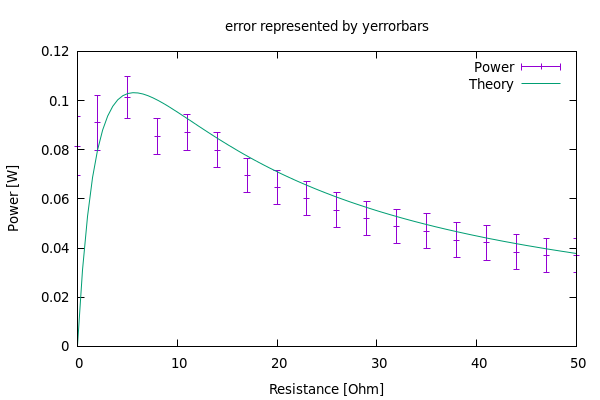
\includegraphics[width=0.9\linewidth]{errorbars1.png}
  \caption{Execution time in seconds.}
  \label{fig:exectime}
\end{figure}

\subsection*{Summary of results}

Table~\ref{tab:results} summarize the results obtained. Please note that the values in the table are only space holders (not the expected execution time).

\begin{table}[h!]
  \centering
    \begin{tabular}{||l r r||} 
    \hline
    Parameter & Average(s) & Standard deviation(s) \\ [0.5ex] 
    \hline
    \hline
    10 & 0.334 & 0.003 \\ 
    50 & 1.235 & 0.034 \\
    100 & etc. & etc. \\
    \hline
    \end{tabular}
  \caption{Summary of results.}
  \label{tab:results}
\end{table}

\end{document}
